\documentclass[11pt]{article}
% \pagestyle{empty}

\setlength{\oddsidemargin}{-0.25 in}
\setlength{\evensidemargin}{-0.25 in}
\setlength{\topmargin}{-0.9 in}
\setlength{\textwidth}{7.0 in}
\setlength{\textheight}{9.0 in}
\setlength{\headsep}{0.75 in}
\setlength{\parindent}{0.3 in}
\setlength{\parskip}{0.1 in}
\usepackage{epsf}
\usepackage{pseudocode}
\usepackage{ amssymb }
\usepackage{tikz}
\usepackage{listings}
\usetikzlibrary{arrows.meta}
\usepackage{algorithmic}
\usepackage{changepage}
\usepackage{lipsum}
\usepackage{enumitem}
\usepackage{indentfirst}
\pagestyle{headings}
\usepackage{graphicx}
\usepackage{amsmath}
\graphicspath{ {desktop/} }
\setlength\parindent{24pt}


% \usepackage{times}
% \usepackage{mathptm}

\def\O{\mathop{\smash{O}}\nolimits}
\def\o{\mathop{\smash{o}}\nolimits}
\newcommand{\e}{{\rm e}}
\newcommand{\R}{{\bf R}}
\newcommand{\Z}{{\bf Z}}
\newcommand{\findent}{\leavevmode{\parindent=2em\indent}}
\newcommand\solution{%
  \textbf{Solution.}\\%
}
\newcommand\floor[1]{\lfloor#1\rfloor}
\newcommand\ceil[1]{\lceil#1\rceil}


\begin{document}

CS 124 Programming Assignment 3 \\
\indent Owen Hakim
\\
\section{\textbf{Problem Definition}}
In this programming assignment we implemented three heuristics for the Number Partition Problem which his NP-complete where the goal is the minimize the residue of the array. Residue is represented as \textit{u} where

\[ u = \sum_{i = 1}^{n} s_{i} * a_{i} \] \\

We implemented each of the three heuristics by calculating the residue of the generated array, and by splitting the set of numbers using the prepartitioning method. \\\\

\section{\textbf{Dynamic Programming Solution}}
The dynamic programming solution to the Number Partition problem runs in \textit{O(ns)} time and uses \textit{O(ns)} space, where \textit{s} is the sum of the integers in \textit{A} and \textit{n} is the length of \textit{A}. The algorithm will return 1 if the given array can be made into two subsets with equal sums (difference is 0), and 0 if it cannot. For a given array \textit{A}, let $T(m,j)$ be 1 if there is a subset of the first \textit{j} elements of \textit{A} which sums to \textit{m}. If the sum of the elements in \textit{A} is \textit{s}, then it is necessary to compute $T(\ceil{s/2}, n)$. If \textit{s} is even then this just equals $s/2$ but if \textit{s} is odd (and thus there is no perfect partition), this will tell us if it’s possible to split \textit{A} into two subsets whose sums differ by 1, which is the best we can do in the odd case. We know that $T(0, i) = 1$ for $0 \leq i \leq n$ because the empty set is a subset of every set and has a sum of zero. The following recurrence will let us calculate $T(\ceil{s/2}, n)$: \\

\begin{equation}
	T(m, j) = \begin{cases}
		1, & \text{$T(m, j - 1} = 1$ or $T(m - A[j], j - 1) = 1$ \\
		0, & \text{otherwise} \\
	\end{cases}
\end{equation}

Essentially, start by figuring out if there’s a subset of the first \textit{j} elements which have a subset that sums to \textit{m}. Either the first $j − 1$ elements could contain such a subset, in which case there would be no need to include $A[j]$ in it, or the first $j − 1$ elements




Let $\textit{A} = (a_1, a_2, ..., a_n)$ where \textit{A} is the given sequence of nonnegative integers. Let \textit{t} be the sum of all
the elements in \textit{A}, which can be represented as  $ \sum_{i=1}^{n} a_{i} $. In this problem, \textit{A} must be divided into two sets, $\textit{A}_1$ and $\textit{A}_2$, where the sum of each set’s elements is as close to half of \textit{t} as possible. This is because for the residue to be as close to 0 as possible, each set needs to have a sum as close to half of the overall sum \textit{t} as possible. This is similar to the subset sum problem (which the number partition problem reduces to), where in this case the sum is equal to half \textit{t}. For the definition of the dynamic programming solution, I let X[i, $\floor{\frac{\textit{t}}{2}}$] be a boolean value, where it is True if there exists a subset of the first \textit{i} numbers of A that add up to $ \floor{\frac{\textit{t}}{2}} $, and False if not. \\\\

\textbf{Recurrence:}\\
\begin{equation}
	T(n) = \begin{cases}
		True, & \text{if $i = 0$ and $\floor{\frac{\textit{t}}{2}} = 0$}. \\
		False, &\text{if $i = 0$ and $\floor{\frac{\textit{t}}{2}} \neq 0$}. \\
		False, &\text{if $i \neq 0$ and $\floor{\frac{\textit{t}}{2}} < 0$}. \\
		X[i - 1, \floor{\frac{\textit{t}}{2}} - a_i] || X[i - 1, \floor{\frac{\textit{t}}{2}}], & \text{otherwise}. \\
	\end{cases}
\end{equation}

For an element $a_i$, first it needs to be determined if it should be included in set $\textit{A}_1$ or $\textit{A}_2$. If set $\textit{A}_1$ is chosen, evaluate X[i - 1, $ \floor{\frac{\textit{t}}{2}} - a_i$] ; if $\textit{A}_2$ is chosen, evaluate X[i - 1, $\floor{\frac{\textit{t}}{2}}$] . This is the recurrence. However, this will also require a table Y[i,s] to determine the actual partitionings. Y[i,s] is None if X[i,s] is False. If X[i,s] is True and X[i - 1, $\floor{\frac{\textit{t}}{2}} - a_i$] is also True, then Y[i,s] stores "$A_1$". If X[i,s] is True and X[i - 1, $\floor{\frac{\textit{t}}{2}} - a_i$] is false, then Y[i,s] stores "$A_2$". Finally, evaluate X[n,b] to see if it is True. If not, move on to X[n,b-1], and then on to X[n,b-2], and then so on until the first instance where it evaluates to True is found. This can be generalized where X[n,b-c] is
the first instance of a True value. Check the second table \textit{Y} at Y[n,b-c]. There are two possibilities of what it will store: "$A_1$" or "$A_2$". If Y[n,b-c] contains "$A_1$", place $a_n$ into set $\textit{A}_1$ recurse on X[i - 1, $\floor{\frac{\textit{t}}{2}} - a_i$]. However,  if [n,b-c] contains "$A_2$", place $a_n$ into set $\textit{A}_1$ and recurse on X[i - 1, $\floor{\frac{\textit{t}}{2}}$]. After this process, there should be two sets, $\textit{A}_1$ and $\textit{A}_2$, each with elements that sum as close to \textit{t} as possible, making the residue as close to 0 as possible. \\\\

\textbf{Time and Space Complexity:}\\
The time complexity is O(nb) since there are O(nb) possible inputs to X and each input takes O(1) time to calculate. Furthermore, the space complexity is also O(nb) since this solution requires the use of both X and Y. \\\\

\section{\textbf{Karmarkar-Karp Runtime}}
The Karmarkarp-Karp algorithm can be implemented in $O(n\log n)$ time by using a max-heap. This section will describe the operations in one iteration of the algorithm. It begins by building a max heap from the array A which takes $O(n\log n)$ time. However, this is not more significant than the run time of the following steps which take $O(n\log n)$ in total. The first step of Karmarkar-Karp is removing the max element which takes O(1) time. This rebalances the heap with MAX-HEAPIFY which takes $O(n\log n)$ time. Removing another max element takes O(1) time and rebalances the heap again with MAX-HEAPIFY, taking $O(n\log n)$ time. Then, it takes the difference of those two elements, which is an arithmetic operation taking O(1) time. In total, one iteration of Karmarkar-Karp takes $O(2\log n)$ time. Then, do \textit{n} iterations of this, where the runtimes can be represented by $2\log n + 2\log{n -1} + 2\log{n-2} + ... + 2\log{1}$. This sequence is equivalent two $O(\frac{2n(\log{n} + \log{1})}{2})$, which simplifies to $O(n\log n)$.  \\\\

\section{\textbf{Results}}
The \textit{kk.py} file runs the Karmarkar-Karp algorithm on an input file of 100 random numbers, as well as the repeated random, hill climbing, and simulated annealing algorithms for both the standard and prepartition representations (which are written in \textit{std\_sol.py} and \textit{prepartition\_sol.py}) for seven results in all. The file prints the residue and runtime for each algorithm. (Note: the  file is compiled with “chmod +x kk.py” and run with “./kk.py <inputfile> ”.) \\\\

The spreadsheet \textit{Progassm3\_results.xlsx} contains the residues and runtimes for he seven methods over 100 random instances of 100 random numbers on the interval [0, $10^12$]. To summarize, here are the averages of the 100 trials for each method.

\indent \textbf{Residues:}\\
\indent \indent \textbf{Karmarkar-Karp:} 258,394.28\\
\indent \indent \textbf{Standard Repeated Random:} 315,334,261.4\\
\indent \indent \textbf{Standard Hill Climbing:} 282,310,367.2\\
\indent \indent \textbf{Standard Simulated Annealing:} 277,117,175.5\\
\indent \indent \textbf{Prepartition Repeated Random:} 180.58\\
\indent \indent \textbf{Prepartition Hill Climbing:} 214.06\\
\indent \indent \textbf{Prepartition Simulated Annealing:} 213.32\\\\

\indent \textbf{Runtimes (in seconds):} \\
\indent \indent \textbf{Karmarkar-Karp:} 0.000483866\\
\indent \indent \textbf{Standard Repeated Random:} 1.005331123\\
\indent \indent \textbf{Standard Hill Climbing:} 0.611045532\\
\indent \indent \textbf{Standard Simulated Annealing:} 0.650936347\\
\indent \indent \textbf{Prepartition Repeated Random:} 12.93445673\\
\indent \indent \textbf{Prepartition Hill Climbing:} 9.819396634\\
\indent \indent \textbf{Prepartition Simulated Annealing:} 9.834228227\\\\

Thee following two graphs represent the residues (logarithmic y-axis scale) and the runtimes for each of the seven methods over the course of 100 trials, respectively.\\
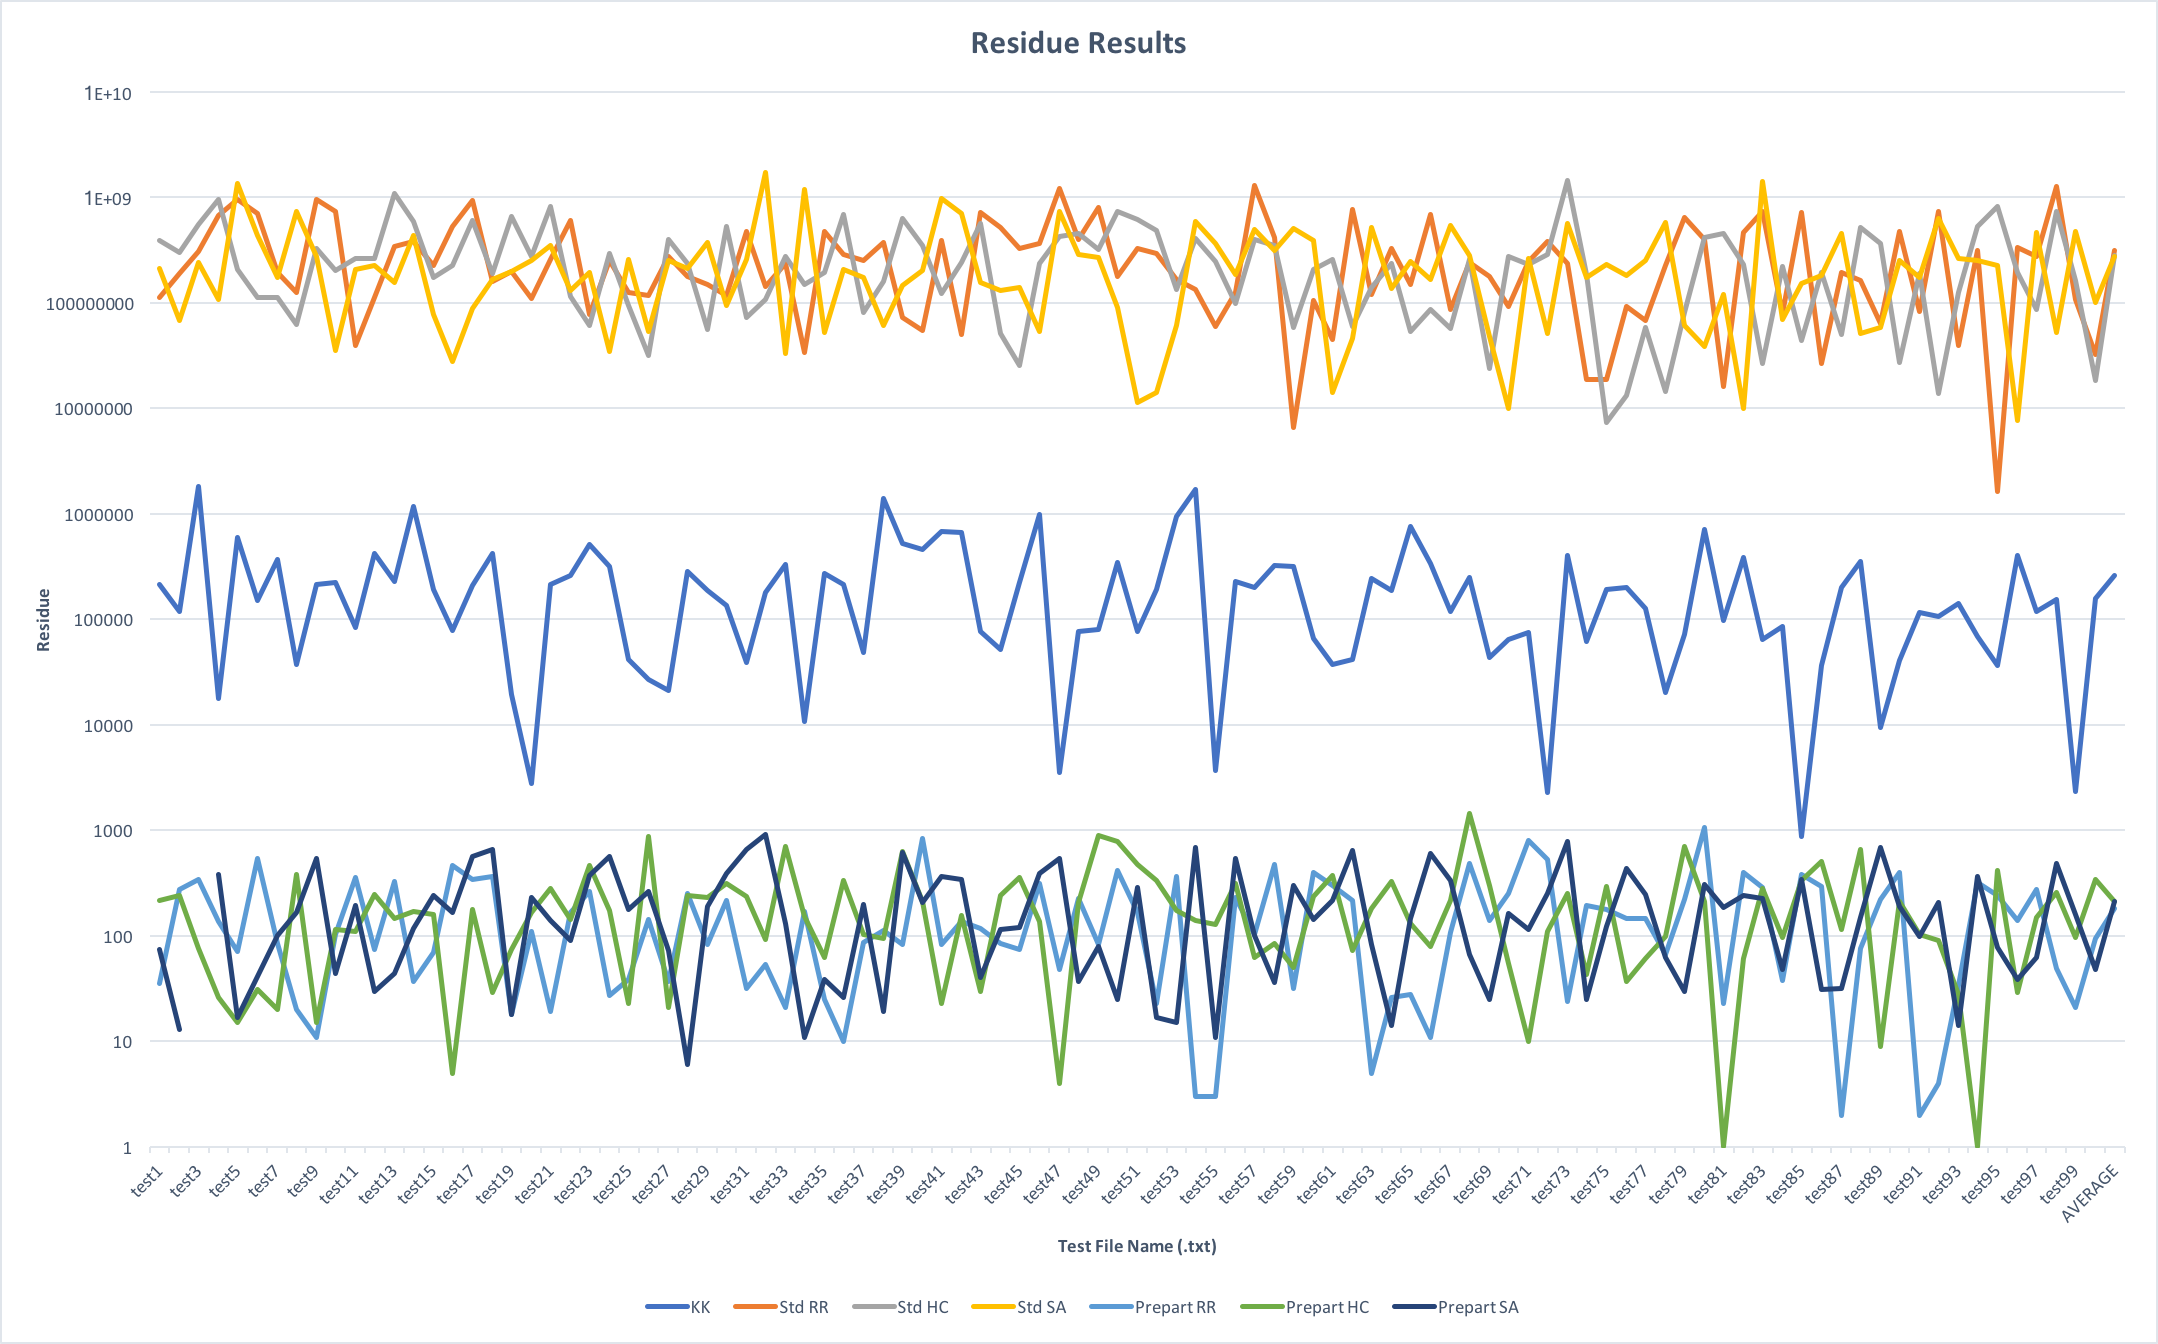
\includegraphics[width=\linewidth]{residueresults}
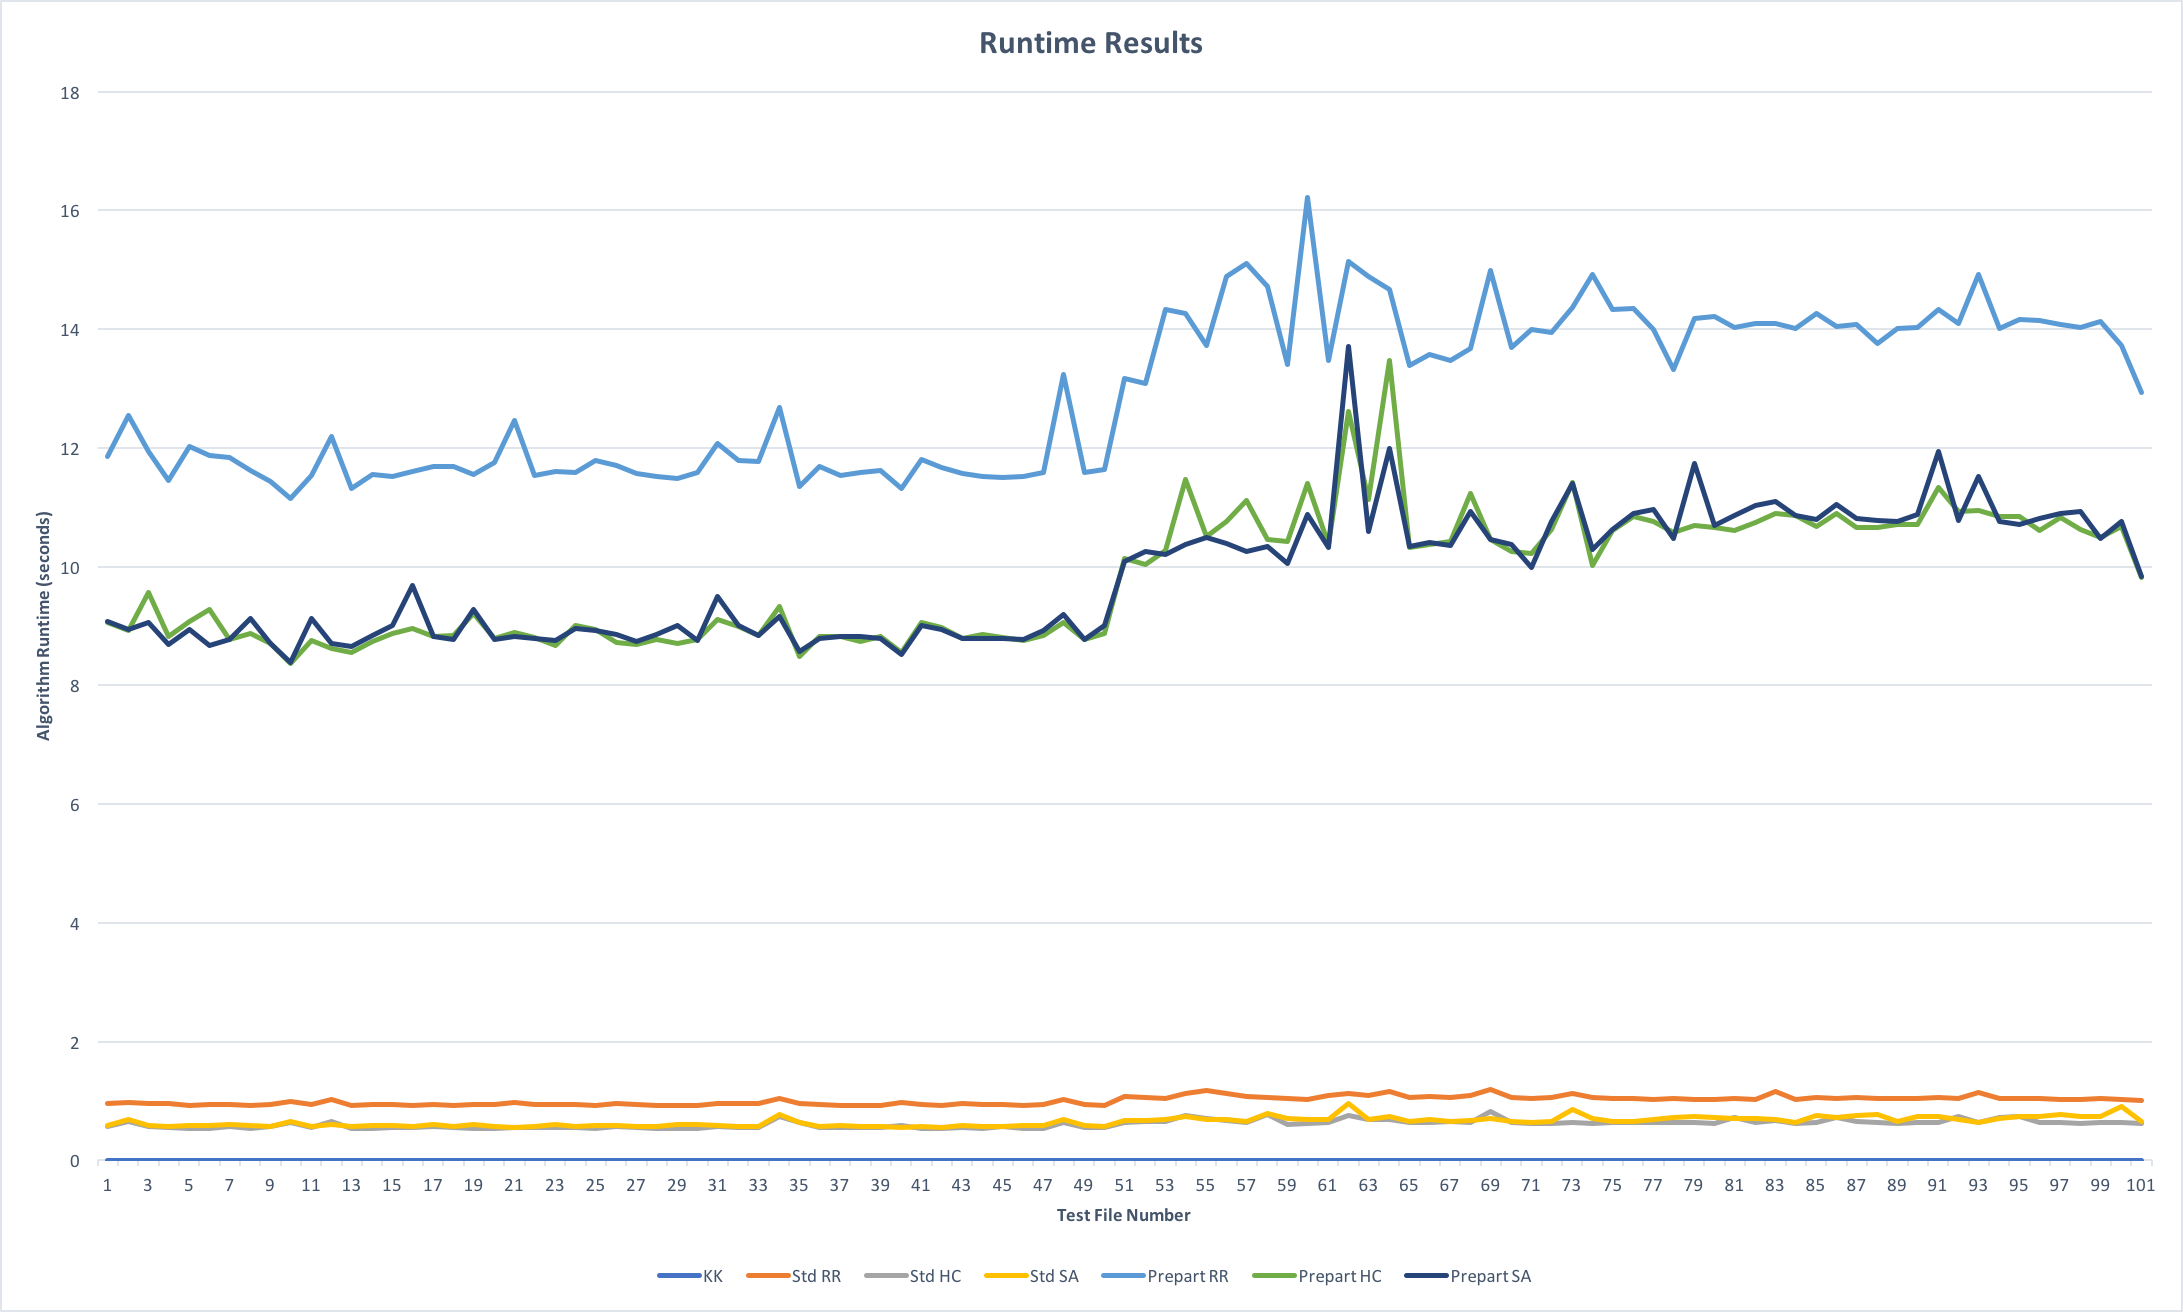
\includegraphics[width=\linewidth]{runtimeresults}

\section{\textbf{Analysis}}
First, consider the results for residues. Looking at the graph, see that the three standard methods’ results are all near each other, as well as the three prepartition methods. The two groups are very far apart, with the prepartition representation giving significantly better results than the standard representation, in the hundreds as opposed to the hundreds of millions. The Karmarkar-Karp algorithm sits in between the two groups, hovering in the hundreds of thousands. \\\\

I expected the prepartition representation to be much more effective than the standard representation because it uses the Karmarkar-Karp heuristic in its algorithms. The KK
algorithm is an effective approximation, giving the prepartition algorithms an advantage in how the lists are represented. Through 25,000 iterations, all of the algorithms under this representation eventually give relatively low and accurate results. The standard representation partitions the given list into two parts at the start, but the prepartitioning representation allows it to be split in a number of partitions up to the number of elements in the set, allowing for more flexibility and efficiency in representing set partitions. Additionally, I expected that Karmarkar-Karp by itself would be somewhere in the middle of the two representations, though the actual results were much closer to those of the prepartition representation than the standard representation to a fairly surprising extent. \\\\

Between the three algorithms, I anticipated that simulated annealing would be the most effective, followed by hill climbing, and then repeated random. In reality, this ordering proved true for the standard representation. However, unexpectedly, the repeated random algorithm was most effective for the prepartition representation by a notable margin. The cause is somewhat unclear, though it may be related to the significant number of iterations run. Because the prepartition representation allows for many different sets to be generated on each iteration, the RR algorithm can eventually find a good solution. Furthermore, the hill climbing was the least effective,
likely due to the algorithm’s tendency to hover around local minima and get stuck. The simulated annealing algorithm avoids this by sometimes jumping to a different location with some decreasing probability, leading to better results. \\\\

As for the runtimes, I expected that the prepartition representation algorithms would take longer than the standard representation due to the need to account for a large number of partitions as opposed to a fixed number in the standard representation. This turned out to be the case, although the stark difference was still surprising. The standard methods took between 0.6 to 1 seconds on average, while the prepartition methods took between 9.8 to 13 seconds on average. Within the prepartition
representation, the HC and SA algorithms took around the same time (9.8 seconds), while the RR algorithm took on average a full 3 seconds longer. Intruigingly, this may be a result of the RR loop constantly generating new partitions to test, as opposed to the HC and SA algorithms generating random neighbor solutions in their loop, a process that takes less time in the long run. Additionally, since Python is known as a relatively slow programming language, these times could possibly be cut down by writing in a lower-level language such as C++. \\\\

Theoretically, the solutions from the investigation of Karmarkar-Karp could be used as a jumping-off point for the other randomized algorithms. Simulated annealing and hill climbing iteratively decrease the residue until the best possible residue is found, so picking a more optimal starting point will give the algorithms a better chance of estimating the true residue. Having used this heuristic, the standard representation algorithms would have likely given much better results for the residue, which is clear from the fact that the prepartition representation used a version of the KK heuristic while the standard representation did not. The prepartition representation algorithm would also likely improve with KK as a starting point, though not as dramatically as the standard representation algorithms. However, using KK as a starting point, it is likely that the repeated random algorithm in either representation would not significantly improve, because it simply generates a new solution each time instead of updating iteratively, so the starting point would not make a major difference.

\end{document}